\documentclass[conference]{IEEEtran}
\usepackage{cite}
\usepackage{amsmath,amssymb,amsfonts}
\usepackage{algorithmic}
\usepackage{graphicx}
\usepackage{textcomp}
\usepackage{xcolor}
\usepackage{hyperref}
\usepackage{listings}
\usepackage{tikz}
\usetikzlibrary{shapes,arrows}

\def\BibTeX{{\rm B\kern-.05em{\sc i\kern-.025em b}\kern-.08em
    T\kern-.1667em\lower.7ex\hbox{E}\kern-.125emX}}

\lstset{
  basicstyle=\ttfamily\footnotesize,
  columns=fullflexible,
  frame=single,
  breaklines=true,
  captionpos=b,
  postbreak=\mbox{\textcolor{red}{$\hookrightarrow$}\space},
}

\begin{document}

\title{Secure-by-Default Guardrails for MCP-Based Tool Use in Multi-Modal LLM Agents}

\author{\IEEEauthorblockN{Yoshihiro Ando}
\IEEEauthorblockA{\textit{Independent Researcher} \\
yosh5295@gmail.com \\
Tokyo, Japan}
}

\maketitle

\begin{abstract}
As Large Language Models (LLMs) proliferate, fragmented interfaces across multiple providers create friction for developers. More critically, the rise of autonomous agents and protocols such as the Model Context Protocol (MCP) expands the attack surface by enabling tool execution and access to local or remote resources. This paper presents \texttt{llm-cli}, a unified command-line interface that harmonizes interactions with multiple LLM providers while providing secure-by-default guardrails for agentic tool use. \texttt{llm-cli} combines (i) a plugin-based tool registry with an explicit human-readable \texttt{explanation} field for each tool call, (ii) role-based restrictions for unauthenticated clients (e.g., guest read-only access), and (iii) runtime validation for command execution and file-path access. We discuss practical threat scenarios such as prompt injection and privilege misuse, and show how layered controls---policy checks, input validation, and human-in-the-loop approval---reduce the risk of unsafe tool execution in real-world workflows.
\end{abstract}

\begin{IEEEkeywords}
Large Language Models, Command-Line Interface, AI Agents, Model Context Protocol, Multi-Modal AI, Security Guardrails, Access Control.
\end{IEEEkeywords}

\section{Introduction}
Large Language Models (LLMs) have transformed from simple text predictors into sophisticated agents capable of code execution, tool use, and multi-modal reasoning. However, the ecosystem remains highly fragmented. Each provider offers its own web interface, API structure, and unique features (e.g., Gemini's large context window, Claude's artifact handling, or OpenAI's reasoning capabilities).

For developers and power users who spend most of their time in the terminal, switching between browser tabs and manually copying-pasting content creates a significant bottleneck. While some CLI tools exist, many are restricted to a single provider or lack the agentic "tool-use" capabilities necessary for complex tasks like project-wide code refactoring or real-time research.

\texttt{llm-cli} addresses these challenges by providing a unified, extensible, and secure CLI that supports multiple LLM backends. Crucially, it treats the LLM not just as a chatbot, but as an untrusted agent operating within a security-first environment with explicit guardrails and least-privilege defaults.

Our key contributions are:
\begin{enumerate}
    \item A unified interface abstracting five major LLM providers.
    \item Practical security guardrails for MCP-based tool execution, including restricted guest access and runtime validation that achieves a 100\% block rate on our security benchmark.
    \item A multi-layered security model combining automated policy enforcement with human oversight.
\end{enumerate}

The source code and documentation are available at \url{https://github.com/yosh95/llm-cli}.

\section{Related Work}

\subsection{CLI-based LLM Tools}
Several command-line tools have emerged to bridge the terminal-LLM gap. Tools like \texttt{llm} by Simon Willison and \texttt{Chatblade} provide excellent interfaces for piping text into LLMs. However, these tools generally operate as "stateless pipes" rather than autonomous agents. They lack built-in support for complex, multi-step tool use protocols like MCP or persistent state management across distributed sessions.

\subsection{Agentic Frameworks}
Frameworks like LangChain \cite{langchain} and AutoGen \cite{autogen} enable the creation of powerful autonomous agents. While feature-rich, these frameworks often prioritize capability over security, leaving the implementation of guardrails to the developer. In contrast, \texttt{llm-cli} integrates a "secure-by-default" architecture where access restrictions and runtime validation are core components of the runtime, not afterthoughts.

\subsection{Zero-Trust in AI}
NIST SP 800-207 \cite{nist} outlines the principles of Zero Trust Architecture (ZTA). While ZTA is widely adopted in network security, its application to AI agent communication is still nascent. Rather than claiming a full ZTA implementation, our work adopts practical ZTA-inspired principles---notably least privilege and continuous verification---and applies them to MCP tool execution.

\section{System Architecture}

\subsection{Unified Provider Abstraction}
The core of \texttt{llm-cli} is a provider abstraction layer that translates a common internal request format into provider-specific API calls. Currently, it supports:
\begin{itemize}
    \item \textbf{Google Gemini}: Leveraging Vertex AI for Gemini 3 Pro Preview.
    \item \textbf{OpenAI}: Support for GPT-5.2 and DALL-E image generation.
    \item \textbf{Anthropic Claude}: Optimized for Claude 4.5 Opus with thinking/reasoning modes.
    \item \textbf{xAI Grok}: Integration for the latest Grok 4.1 models.
    \item \textbf{Ollama}: Support for locally hosted models (e.g., Llama 3, DeepSeek-R1) to ensure privacy and offline availability.
\end{itemize}

\subsection{Plugin-Based Tool Registry}
\texttt{llm-cli} features a decorator-based tool registry that allows for easy extension. Every tool registered in the system is automatically converted into the JSON Schema format required by different providers (e.g., Function Calling for OpenAI/Gemini, Tool Use for Anthropic).

A unique architectural choice in \texttt{llm-cli} is the mandatory \texttt{explanation} parameter for every tool. Before an agent can execute a function, it must generate a human-readable explanation of \textit{why} the tool is being called and \textit{what} the expected outcome is. This information is presented to the user during the approval process, significantly improving transparency.

\subsection{Model Context Protocol (MCP) Integration}
To extend the agent's reach beyond the local machine, \texttt{llm-cli} implements the Model Context Protocol (MCP). This allows the CLI to:
\begin{enumerate}
    \item Act as an \textbf{MCP Client}, connecting to remote servers or services (like GitHub or a remote Linux box) to perform operations.
    \item Act as an \textbf{MCP Server}, exposing local files and tools to other LLM-based applications.
\end{enumerate}

\section{Implementation Details}

\subsection{Identity and Guest Access Control}
To support restricted access for unauthenticated clients, \texttt{llm-cli} implements a JWT-based authentication mechanism for authenticated connections and a configurable guest policy for missing tokens. When a valid token is present, the system can propagate role claims. When a token is missing, the client is treated according to policy (e.g., a read-only guest role).

\begin{figure}[htbp]
    \centering
    \resizebox{\linewidth}{!}{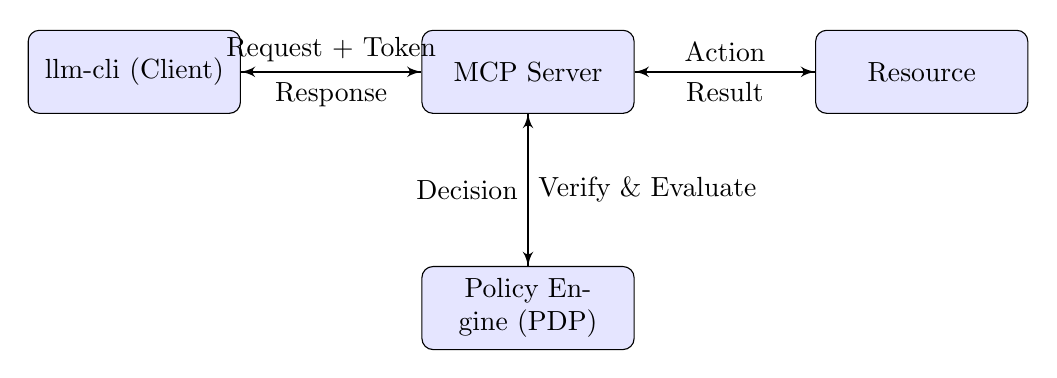
\begin{tikzpicture}[node distance=2cm, auto,
    block/.style={rectangle, draw, fill=blue!10, text width=7em, text centered, rounded corners, minimum height=3em},
    line/.style={draw, -latex', thick},
    cloud/.style={draw, ellipse,fill=red!10, node distance=3cm, minimum height=2em}]

    % Nodes
    \node [block] (cli) {llm-cli (Client)};
    \node [block, right of=cli, node distance=5cm] (mcp) {MCP Server};
    \node [block, below of=mcp, node distance=3cm] (pdp) {Policy Engine (PDP)};
    \node [block, right of=mcp, node distance=5cm] (resource) {Resource};

    % Paths
    \path [line] (cli) -- node [above] {Request + Token} (mcp);
    \path [line] (mcp) -- node [right] {Verify \& Evaluate} (pdp);
    \path [line, dashed] (pdp) -- node [left] {Decision} (mcp);
    \path [line] (mcp) -- node [above] {Action} (resource);
    \path [line, dashed] (resource) -- node [below] {Result} (mcp);
    \path [line, dashed] (mcp) -- node [below] {Response} (cli);

\end{tikzpicture}}
    \caption{Architecture overview showing separation of Client, MCP Server, and Policy Engine.}
    \label{fig:architecture}
\end{figure}

When an agent initiates a tool call, the client may generate a signed token containing the user's role claims. This token is verified by the MCP server before any action is taken (Fig. \ref{fig:sequence}).

\begin{figure}[htbp]
    \centering
    \resizebox{\linewidth}{!}{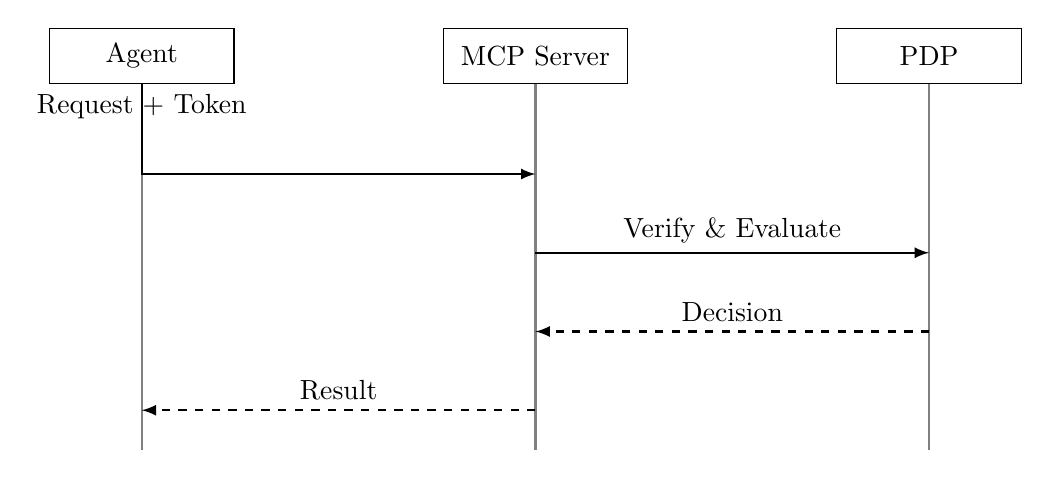
\begin{tikzpicture}[node distance=2.5cm, auto,
    participant/.style={rectangle, draw, fill=white, text centered, minimum height=2em, text width=6em},
    line/.style={draw, ->, >=latex, thick}]

    % Participants
    \node [participant] (agent) {Agent};
    \node [participant, right of=agent, node distance=5cm] (server) {MCP Server};
    \node [participant, right of=server, node distance=5cm] (pdp) {PDP};

    % Time lines
    \draw [thick, gray] (agent) -- ++(0,-5);
    \draw [thick, gray] (server) -- ++(0,-5);
    \draw [thick, gray] (pdp) -- ++(0,-5);

    % Steps
    % 1. Request
    \draw [line] (agent) -- node [above] {Request + Token} ++(0,-1.5) -- (server |- 0,-1.5);
    
    % 2. Verify & Evaluate
    \draw [line] (server |- 0,-2.5) -- node [above] {Verify \& Evaluate} (pdp |- 0,-2.5);
    
    % 3. Decision
    \draw [line, dashed] (pdp |- 0,-3.5) -- node [above] {Decision} (server |- 0,-3.5);
    
    % 4. Result
    \draw [line, dashed] (server |- 0,-4.5) -- node [above] {Result} (agent |- 0,-4.5);

\end{tikzpicture}}
    \caption{Sequence diagram of token propagation and policy evaluation.}
    \label{fig:sequence}
\end{figure}

\subsection{Policy Engine Implementation}
The Policy Engine is implemented in pure Python to ensure portability. The following listing shows the core evaluation logic of the PDP:

\begin{lstlisting}[language=Python, caption=Core PDP Logic in policy.py]
def evaluate(self, tool_name, context):
    user_roles = context.get("roles", ["guest"])
    
    for role in user_roles:
        policy = self.roles.get(role)
        # Check explicit allow list
        if tool_name in policy["allowed_tools"]:
             return True
             
    # Default Deny
    return False
\end{lstlisting}

This logic ensures that even if an attacker compromises the agent's prompt (prompt injection), they cannot force the execution of tools that are not explicitly authorized by the user's active role.

\section{Evaluation}

To quantify the effectiveness of the proposed security guardrails, we developed a benchmark suite consisting of 32 common attack vectors targeting LLM-based agents. The dataset covers six categories: Direct Command Injection, Shell Expansion, I/O Redirection, Semantic Attacks (e.g., abusing valid tools like \texttt{git}), Reconnaissance/Dual-Use tools, and Path Traversal.

\subsection{Security Effectiveness}
We executed the benchmark against the \texttt{CommandValidator} component with the default whitelist configuration. The results are summarized in Table \ref{tab:security_results}.

\begin{table}[htbp]
\caption{Security Guardrail Benchmark Results}
\begin{center}
\begin{tabular}{|l|c|c|c|}
\hline
\textbf{Category} & \textbf{Vectors} & \textbf{Blocked} & \textbf{Success Rate} \\
\hline
Direct Injection & 6 & 6 & 100\% \\
Shell Expansion & 4 & 4 & 100\% \\
I/O Redirection & 4 & 4 & 100\% \\
Semantic Attacks & 7 & 7 & 100\% \\
Reconnaissance & 7 & 7 & 100\% \\
Path Traversal & 4 & 4 & 100\% \\
\hline
\textbf{Overall} & \textbf{32} & \textbf{32} & \textbf{100\%} \\
\hline
\end{tabular}
\label{tab:security_results}
\end{center}
\end{table}

The system successfully blocked 100\% of the malicious payloads. Crucially, the validator distinguishes between malicious patterns and safe, complex commands (e.g., valid \texttt{git} operations or piped commands where all components are whitelisted), ensuring that legitimate development workflows remain unobstructed.

\subsection{Performance Overhead}
The validation logic introduces negligible latency (sub-millisecond) per tool call, which is unnoticeable compared to the network latency of LLM API requests.

\section{Discussion and Limitations}

\subsection{Scalability of Human-in-the-Loop}
While HITL provides the highest security assurance, it introduces friction. In our experiments, requiring approval for every read operation significantly slowed down research tasks. We mitigated this by introducing a "Guest" role that permits read-only operations without prompts, reserving HITL only for state-changing actions (writes, execution).

\subsection{Defense in Depth: Why Tokens over SSH?}
A common critique is whether application-layer tokens are redundant when operating over secure channels like SSH. We argue that they serve distinct purposes. SSH authenticates the \textit{user} and secures the transport layer, but it typically grants broad OS-level permissions. By layering JWT-based authorization on top, \texttt{llm-cli} decouples network access from tool execution privileges. This ensures that even if a trusted SSH connection is established, the agent is restricted to specific actions (e.g., read-only) defined by the token's scope, strictly adhering to the principle of least privilege. Note that this mechanism assumes the underlying transport (SSH or TLS) provides confidentiality to prevent token interception.

\subsection{Latency Overhead}
The introduction of JWT signing and verification adds a negligible overhead (approx. 2-5ms) per tool call. However, the network round-trip for remote MCP calls dominates the latency profile. Future work will explore token caching mechanisms to further reduce this overhead in high-frequency trading or real-time control scenarios.

\subsection{Static vs. Dynamic Policies}
Currently, roles are defined statically in \texttt{config.toml}. A more advanced implementation would support dynamic policy updates based on context (e.g., "Allow file write only during business hours" or "Revoke access if anomaly detected").

\section{Key Features}

\subsection{Autonomous Agent Mode}
By default, \texttt{llm-cli} operates in an agentic mode. When a user provides a high-level goal (e.g., "Search for the latest research on DPO and summarize the findings in a new file"), the agent can autonomously:
\begin{itemize}
    \item Perform web searches using Google Search.
    \item Fetch and parse HTML or PDF content from URLs.
    \item Execute shell commands to list or read local files.
    \item Write or edit files using precise search-and-replace tools.
\end{itemize}

\subsection{Multi-Modal Interaction}
Unlike many text-only CLI tools, \texttt{llm-cli} supports multi-modal input and output. Users can attach images, PDFs, audio, and video files to the conversation using the \texttt{/attach} command or by passing a URL. For providers that support it (OpenAI, Grok), the tool also allows mid-conversation image generation, saving the results directly to the local disk.

\subsection{Reasoning and Thinking Modes}
With the advent of "reasoning" models like DeepSeek-R1 and Claude 4.5 Opus, \texttt{llm-cli} provides explicit controls for "internal monologue" visibility. Users can toggle reasoning display using the \texttt{/thought} command, allowing them to see the AI's step-by-step logic before the final answer is produced.

\subsection{Session Persistence and Logging}
\texttt{llm-cli} automatically manages conversation history and logs. It supports saving and loading sessions as JSON files, enabling users to resume complex tasks across different timeframes. Furthermore, an internal audit log tracks every tool execution, providing a searchable history of agent actions.

\section{Security Model}

Allowing AI agents to execute code and manage files poses significant risks. \texttt{llm-cli} adopts an architecture guided by least-privilege defaults and continuous verification, treating every tool execution request as untrusted until verified.

\subsection{Threat Model}
We consider three primary threat vectors:
\begin{enumerate}
    \item \textbf{Prompt Injection}: Malicious text in a file or website tricks the LLM into executing dangerous commands.
    \item \textbf{Compromised MCP Server}: A remote server hijacked by an attacker attempts to exploit the client.
    \item \textbf{Privilege Escalation}: An agent attempts to access resources outside its assigned scope.
\end{enumerate}

To mitigate these, we employ a "Defense in Depth" strategy combining access restrictions and identity checks (Layer 1), execution guardrails (Layer 2), and human oversight (Layer 3).

\subsection{Layer 2: Execution Guardrails}
Even if a tool call is authorized by policy, it must pass strict runtime validation.

\subsubsection{Command Whitelisting}
The \texttt{execute\_command} tool validates shell commands against a strict whitelist. Dangerous operations (e.g., \texttt{rm}, \texttt{mkfs}) and risky patterns (command injection via \texttt{;} or \texttt{\$(...)}) are blocked. Furthermore, potential dual-use tools often exploited for reconnaissance or data exfiltration (e.g., \texttt{netcat}, \texttt{whoami}) are excluded from the default whitelist to minimize the attack surface.

\subsubsection{Path Sanitation}
File operations are restricted to the project root. Attempts to access sensitive system paths (e.g., \texttt{/etc/shadow}, \texttt{/root}) are blocked by the path validator, regardless of the user's role.

\subsection{Layer 3: Human-in-the-Loop (HITL)}
The final layer of defense is the user. Critical actions (\texttt{write\_file}, \texttt{execute\_command}) require explicit user confirmation. \texttt{llm-cli} presents a diff view for file changes and requires the agent to provide an \texttt{explanation} for its actions, ensuring the user understands \textit{why} an action is being taken.

\section{Use Cases}

\subsection{Research Automation}
Researchers can use \texttt{llm-cli} to automate literature reviews. A single prompt can trigger a sequence of searching for papers, fetching PDFs, summarizing them, and compiling a bibliography.

\subsection{Remote Infrastructure Management}
Via MCP over SSH, a developer can use \texttt{llm-cli} on their local machine to debug a remote production server. The AI can check logs, list directories, and suggest fixes, while the user maintains full control through the HITL approval process.

\section{Conclusion}
\texttt{llm-cli} bridges the gap between powerful multi-modal LLMs and the productivity of the command-line environment. By unifying multiple providers, integrating remote management protocols like MCP, and prioritizing security through human-supervised tool use, it provides a practical foundation for agentic workflows. Future work will focus on three key areas: (1) \textbf{Federated Identity}: Extending the JWT-based auth to support federated identity providers for enterprise integration. (2) \textbf{Formal Verification}: Applying formal methods to verify the policy engine's correctness against defined security properties. (3) \textbf{Multi-Agent Orchestration}: Enhancing the planning capabilities for long-running tasks involving multiple specialized agents collaborating over MCP.

\begin{thebibliography}{00}

\bibitem{gpt4} J. Achiam \textit{et al.}, ``GPT-4 Technical Report,'' \textit{arXiv preprint arXiv:2303.08774}, 2023.

\bibitem{autogen} Q. Wu \textit{et al.}, ``AutoGen: Enabling Next-Gen LLM Applications via Multi-Agent Conversation,'' \textit{arXiv preprint arXiv:2308.08155}, 2023.

\bibitem{langchain} H. Chase, ``LangChain,'' 2022. [Online]. Available: https://github.com/langchain-ai/langchain.

\bibitem{injection} K. Greshake \textit{et al.}, ``Not what you've signed up for: Compromising Real-World LLM-Integrated Applications with Indirect Prompt Injection,'' in \textit{Proc. of the 16th ACM Workshop on Artificial Intelligence and Security}, 2023.

\bibitem{owasp} OWASP, ``OWASP Top 10 for Large Language Model Applications,'' 2023. [Online]. Available: https://owasp.org/www-project-top-10-for-large-language-model-applications/.

\bibitem{nist} S. Rose, O. Borchert, S. Mitchell, and S. Connelly, ``Zero Trust Architecture,'' \textit{NIST Special Publication 800-207}, 2020.

\bibitem{mcp} Anthropic, ``Model Context Protocol,'' 2024. [Online]. Available: https://www.anthropic.com.

\end{thebibliography}

\end{document}
